\chapter{Projekt}\label{chap:proj}\lstset{language=C++}
Rozdział ten zawiera inżynierski projekt rozwiązań dla wymagań z~poprzednich rozdziałów. Poza opisem tekstowym, zastosowałem w~nim diagramy klas oraz sekwencji UML.

\section{Podział na warstwy}
Zdecydowałem się podzielić wykres na pięć warstw. Odrysowywanie wykresu polega na odrysowaniu zawartości każdej z~warstw, począwsze od tła, a~na pierwszym planie skończywszy.
Układ warstw został przedstawiony na rysunku~\ref{rys:warstwy}.

\begin{figure}[H]
\centering
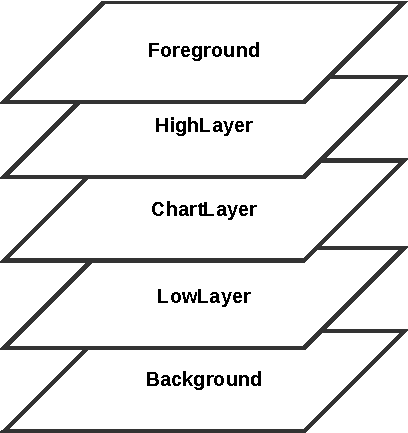
\includegraphics{img/warstwy.pdf}
\caption{Warstwy wykresu}\label{rys:warstwy}
\end{figure}

Warstwy tła oraz pierwszego planu służą jedynie odrysowywaniu wzorów przekazanych za pomocą pędzla. Pozostałe warstwy są bardziej złożone i~zawierają liczne elementy.

Warstwy niska i~wysoka są odrysowywane zgodnie z~algorytmem malarza. Służą dodawaniu przez programistów własnych elementów do wykresów istniejących klas.

Warstwa wykresu służy odrysowaniu głównej zawartości wykresu. Tym etapem steruje strategia danego wykresu. W~ogólnym przypadku programiści nie powinni dodawać własnych elementów do tej warstwy.

%\subsection{Metoda szablonowa}
Metoda odpowiedzialna za odrysowywanie wykresu jest \textit{Metodą Szablonową}~\cite{Patterns}, czyli niewirtualną, publiczną metodą klasy bazowej, wywołującą kolejne metody odpowiedzialne za odrysowanie pojedynczych warstw. Metody te są wirtualne i~chronione.
Metody odpowiedzialne za tło i~pierwszy plan udostępniają domyślną implementację, natomiast pozostałe są czysto wirtualne.

\section{Lokalny układ współrzędnych}
Każdy z~wykresów posiada lokalny, kartezjański układ współrzędnych rzeczywistych. Ponadto granice wykresu są wyznaczane przez specjalny prostokąt. Takie podejście umożliwi układanie elementów względem lokalnego, a~nie globalnego układu współrzędnych, oraz ustalanie, które z~elementów są widoczne i~należy je odrysować. Dodatkowo ułatwiona to realizację takich wymagań jak: skalowanie wykresu czy interaktywność. 

\begin{figure}[H]
\centering
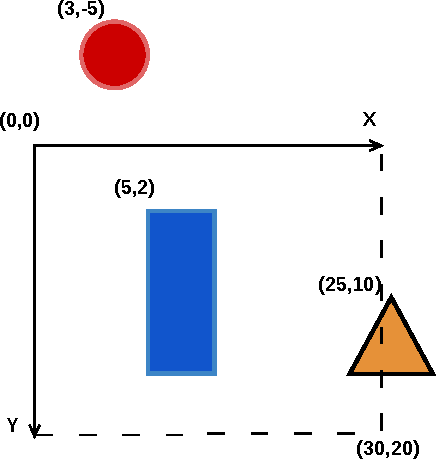
\includegraphics{img/uklad_wspolrzednych.pdf}
\caption{Lokalny układ współrzędnych}\label{rys:uklad:wspolrzednych}
\end{figure}

Na rysunku~\ref{rys:uklad:wspolrzednych} przedstawiono przykładowy układ współrzędnych wykresu o~wymiarach 30x20. W~tej sytuacji prostokąt zostanie wyświetlony w~całości, trójkąt tylko częściowo, a~koło wcale nie zostanie wyświetlone.


\section{Struktura wykresu}
Ogólna koncepcja na strukturę wykresu została przedstawiona na diagramie~\ref{rys:klasy:top_level}.

Klasy pochodne od QocAbstractChart są miejscem łączącym wszystkie inne elementy. To na nich są ustawiane parametry odnoszące się do całości wykresu, np. włączenie antyaliasingu.

QocSeries odpowiada za dane dostarczane do wykresu. Jest lekkim odpowiednikiem modelu z~architektury Model-Widok.

QocAbstractStrategy to klasa bazowa dla strategii -- layoutu, odpowiedzialnego za odpowiednie układanie elementów wykresu, głównie z~warstwy środkowej -- \textit{ChartLayer}, i~ich odrysowywanie. Jest to szczególnie przydatny komponent dla wykresów, które mogą być budowane na różne sposoby, np. wykres słupkowy.


\begin{figure}[H]
\centering
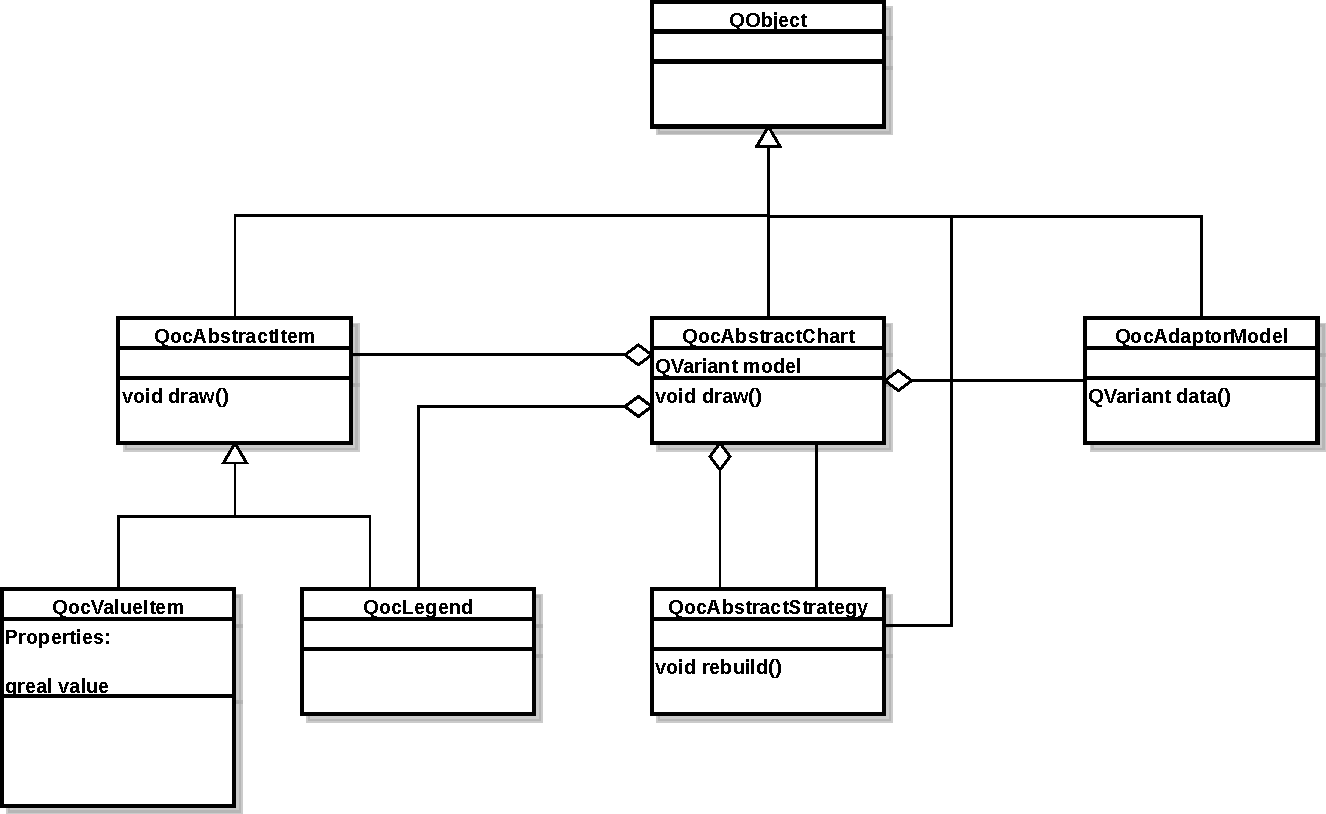
\includegraphics[scale=0.7]{img/klasy-top_level.pdf}
\caption{Diagram top level}\label{rys:klasy:top_level}
\end{figure}

\section{Źródła danych}\label{sec:zrodla}

Jako że źródłem danych dla wykresu może być seria danych, lista serii albo model, postanowiłem wprowadzić pośrednią klasę, która będzie odpowiedzialna za unifikację komunikacji wykresu ze źródłem danych. Klasa ta jest \textit{Adapterem obiektowym}~\cite{Patterns} -- agreguje źródła danych dostarczane jako obiekty \textit{QVariant}. Hierarchię klas związanych z~adapterem przedstawiłem na diagramie~\ref{rys:adapter:model}

\begin{figure}[H]
\centering
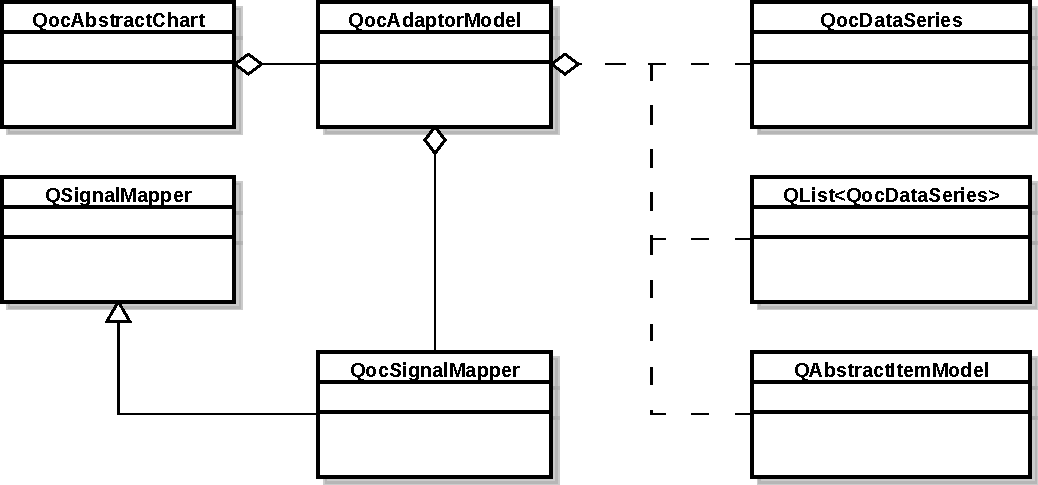
\includegraphics[scale=0.8]{img/adapter-model.pdf}
\caption{Adapter}\label{rys:adapter:model}
\end{figure}

Za pomocą adaptera uzyskałem pewną abstrakcję, dzięki której niezależnie od klasy źródła danych, wykres zawsze będzie go postrzegał jako zbiór serii. Większość metod adaptera, jako jeden z~argmuentów przyjmuje numer serii, dzięki któremu można wyspecyfikować, której serii dotyczy dana operacja. 

Komunikacja w~drugą stronę została rozwiązana za pomocą zbioru sygnałów, które również niosą informację o~numerze serii. W~przypadku zbioru serii, wystarczy uzupełnić ich sygnały o~numer serii oraz przepropagować na zewnątrz adaptera. Chcę to osiągnąć za pomocą obiektu klasy pochodnej od \textit{QSignalMapper}~\footnote{QSignalMapper \url{http://qt-project.org/doc/qt-5.0/qtcore/qsignalmapper.html}}. W~przypadku klas modeli, również muszę wykonać podobne mapowanie, podczas którego trzeba sięgnąć do modelu po numer serii. Przykładowy protokół komunikacji wykresu z~adapterem przedstawiłem na rysunku~\ref{rys:wykres:model}.

\begin{figure}[H]
\centering
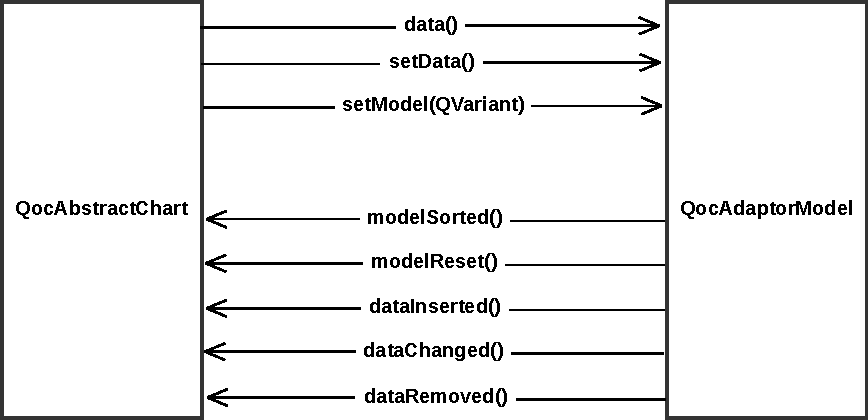
\includegraphics[scale=0.8]{img/wykres-model.pdf}
\caption{Komunikacja Wykres -- Adapter}\label{rys:wykres:model}
\end{figure}

\subsection{Role}
Wzorując się na systemie Model-Widok, zdecydowałem się wprowadzić do mojej biblioteki byt o~nazwie: Rola. Rola to typ wyliczeniowy, który służy do wskazania przez widok, jakich danych oczekuje od modelu. Widok chcąc uzyskać dane z~modelu musi mu przekazać indeks i~właśnie rolę.

Dzięki rolom uzyskałem stan, w~którym wykres chcąc pobrać dane z~modelu, przekazuje do adaptera rolę. Adapter zajmuje się przetłumaczeniem roli. W~zależności od kontekstu, może to być numer kolumny, rola  albo właściwość obiektu.

\begin{lstlisting}[caption=Rola -- typ wyliczeniowy, label=code:role]
enum Role{
	XRole,
	YRole,
	TitleRole,
	ColorRole,
	CustomRole
}
\end{lstlisting}

%Każda z~wartości tego~\ref{code:role} typu wyliczeniowego musi posiadać odpowiadający jej łańcuch znaków. Dwukierunkowe mapowanie wartości oraz łańcuchów umożliwi korzystanie z~serii w~QML, w~sposób analogiczny do modeli.


\subsection{Seria danych}
Źródłem danych dla wykresu może być pojedyncza seria lub lista serii. Aby było to możliwe, typy \textit{QocSeries} i~ \textit{QList<QocSeries>} muszą zostać zarejestrowane jako \textit{QVariant}.

Próbka to w~dużej mierze mapa, w~której kluczem jest rola. Dzięki wsparciu QML dla tego typu map~\footnote{Typ variant\url{http://qt-project.org/doc/qt-5.0/qtqml/qml-variant.html\#storing-\newline arrays-and-objects}} modyfikacja zawartości próbki jest tak samo prosta i~intuicyjna w~C++ oraz w~QML. Diagram~\ref{rys:seria} zawiera najważniejsze elementy klas odpowiedzialnych za serie oraz próbki w~mojej bibliotece.

\begin{figure}[H]
\centering
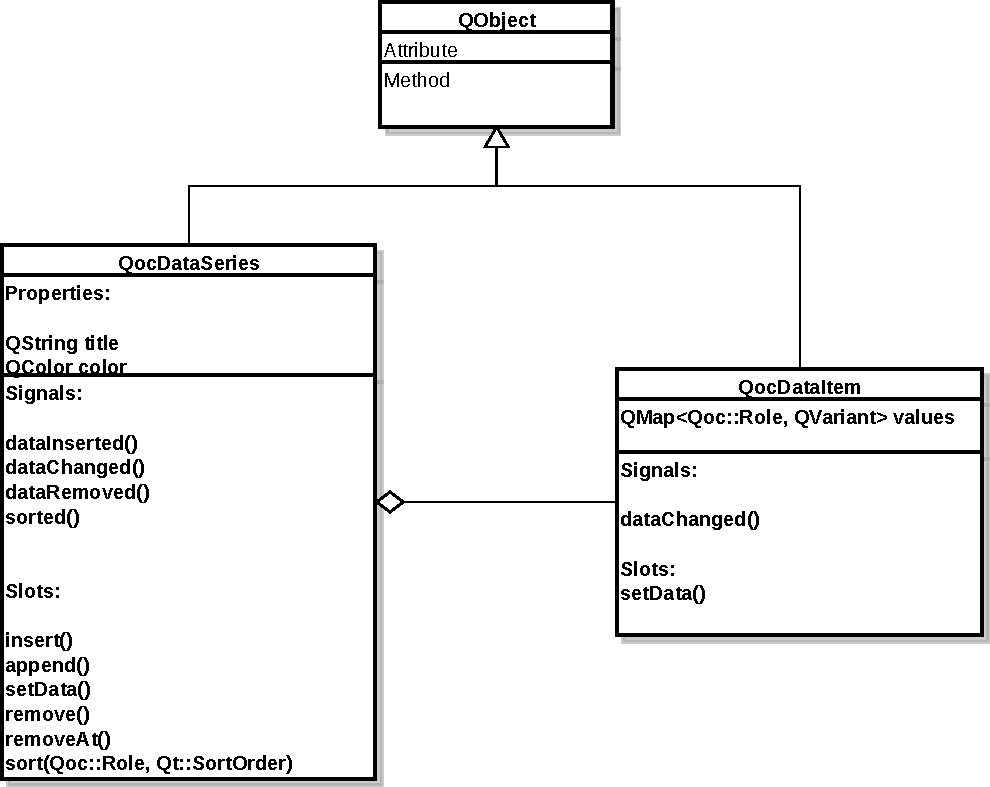
\includegraphics[scale=0.8]{img/seria_danych.pdf}
\caption{Seria i próbki}\label{rys:seria}
\end{figure}

\subsection{QAbstractItemModel}
Pracując na seriach danych, które są mojego autorstwa, mogę założyć, że dla elementu o~danym indeksie i~roli wartość jest, np. tytułem zapisanym w~łańcuchu znaków. Takiego komfortu jednak nie będzie przy współpracy z~dowolnym innym modelem. Nie mogę wymagać od użytkownika, aby interesujące mnie dane trzymał w~kolumnach o~ustalonych przeze mnie indeksach. Rozwiązaniem tej sytuacji mogłoby być stworzenie specjalnego proxy modelu~\footnote{Proxy modele \url{http://qt-project.org/doc/qt-5.0/qtcore/qabstractproxymodel.html}}, jednak preferuję inny sposób.

Moje rozwiązanie polega na mapowaniu ról, które są zrozumiałe dla wykresów, na numery kolumn modeli do tych wykresów podłączanych. W~przypadku jednowymiarowych modeli dziedziczących po \textit{QAbstractListModel} role wykresu będą mapowane na role tychże modeli. Z~perspektywy programisty mapowanie ogranicza się jedynie do wywołania poniższej metody dla wszystkich wymagających tego ról:

\begin{lstlisting}
QocAbstractChart::
setRoleMapping(Qoc::Role role, int customValue);
\end{lstlisting}

Metoda ta przyjmuje jako pierwszy z~argumentów rolę, a~jako drugi numer kolumny, pod którą kryją się odpowiednie dane w~modelu.


\subsection{QML}
ListModel i XmlListModel to pochodne \textit{QAbstractListModel}, które należy potraktować osobno. Wprowadzają one bardziej obiektowe podejście, dzięki czemu ich zawartość jest łatwo dostępna z~QML.

Dane z~tych modeli są dostępne również poprzez system właściwości. Aby dostać się do wartości właściwości wystarczy jedynie znać jej nazwę. Dzięki temu, wymuszając na użytkownikach określone nazwy właściwości, jestem w~stanie pobierać dane z~ich modeli. W~skrajnym przypadku, gdy programista korzystający z~mojej biblioteki nie będzie mógł dostarczyć danych w~oczekiwanym przeze mnie formacie, udostępniam mu przeładowaną metodę z~poprzedniego podpunktu:

\begin{lstlisting}
QocAbstractChart::
setRoleMapping(Qoc::Role role, const QString &name);
\end{lstlisting}

W~tym przypadku jako drugi argument przyjmuję nową nazwę danej właściwości. Po wywołaniu metody, nowa nazwa właściwości będzie wykorzystywana do komunikacji z~modelem.


\section{Qt Quick}
Wykorzystanie mojej biblioteki w~Qt~Quick wymaga pewnego narzutu pracy. Poniżej opisuję mechanizm umożliwiający wykorzystanie moich klas w~QML oraz przyjętą przeze mnie konwencję interfejsów dla QML.

\subsection{Eksport klas C++ do QML}
Klasy wszystkich wysokopoziomowych elementów są pochodnymi klasy QObject. Wszelkie ich parametry, które powinny być konfigurowalne dla programistów włączyłem do zbioru właściwości tych klas. Ważne jest, aby przy zmianie wartości danej właściwości, i~tylko wtedy, emitować sygnał informujący o~tym zdarzeniu. Jest to niezbędne do poprawnego działania mechanizmu wiązania w~QML. Ponadto, wszystkie metody, które powinny być dostępne z~QML, a~nie są slotami, zostają opatrzone makrem \textit{Q\_INVOKABLE}.

Większość klas powinna jest gotowa do wyeksportowania ich do QML za pomocą standardowej procedury, np. poprzez wywołanie funkcji szablonowej
\begin{lstlisting}
template<typename T>
int qmlRegisterType(const char *uri, int versionMajor, 
		    int versionMinor, const char *qmlName)
\end{lstlisting}
Parametrem szablonu jest eksportowany typ, a~parametry funkcji to nazwa modułu, dwie liczby odpowiadające za wersję modułu oraz nazwa pod jaką będzie dostępna eksportowana klasa z~poziomu QML. Qt udostępnia jeszcze kilka innych, specjalizowanych szablonów, np. dla singletonów.

Pozostałe klasy, do wykorzystania ich w~QML, będą wymagają specjalnych interfejsów. Dla klas związanych z~GUI, bazujących na QPainter będzie to QQuickPaintedItem, a~dla tych wykorzystujących SceneGraph -- QQuickItem.

\subsection{Uproszczony interfejs}
Aby zapobiec nadmiernemu rozrostowi interfejsów klas dostępnych w~QML, zdecydowałem się je uprościć w~porównaniu do tych dostępnych z~poziomu C++. Jest to konwencja szeroko stosowana w~QML. Najlepszym przykładem będzie ramka wokół prostokąta. Z~poziomu C++ istnieje możliwość ustawienia pióra używanego do jej odrysowania. Klasa pióra, czyli \textit{QPen}, nie dziedziczy po \textit{QObject}, więc nie może być dostępna w~QML. W~QML można zmienić jedynie kolor oraz grubość ramki.

\section{Interaktywność}
Wszystkie operacje interaktywne zostały rozwiązane za pomocą systemu zdarzeń Qt~\footnote{System zdarzeń Qt \url{http://qt-project.org/doc/qt-5.0/qtcore/eventsandfilters.html}}. Widoki mają obowiązek przekazywać wszelkie przeznaczone dla wykresu zdarzenia, np. pojawienie się kursora myszy nad wykresem czy kliknięcie.

\subsection{Zaznaczanie}
Aby zrealizować zaznaczanie elementów wykresu z~poziomu GUI, do wykresu muszą być przekazywane zdarzenia związane z~kursorem myszy oraz dotykiem. Pojedyncze kliknięcie w~element reprezentujący dane skutkuje jego zaznaczeniem. Podwójne kliknięcie takiego elementu spowoduje zaznaczenie wszystkich elementów danej serii. Zaznaczenie powoduje zmianę koloru obramowania wokół danego elementu. Kolor zaznaczenia jest zdefiniowany jako właściwość całego wykresu.

\subsection{Zmiana wartości w modelu}
Na rysunku~\ref{rys:seq:inter} przedstawiam diagram sekwencji dotyczący zmiany zawartości modelu poprzez modyfikację elementów widoku. Przerywane strzałki zawierające opis symbolizują wywołanie sygnału.

\begin{figure}[H]
\centering
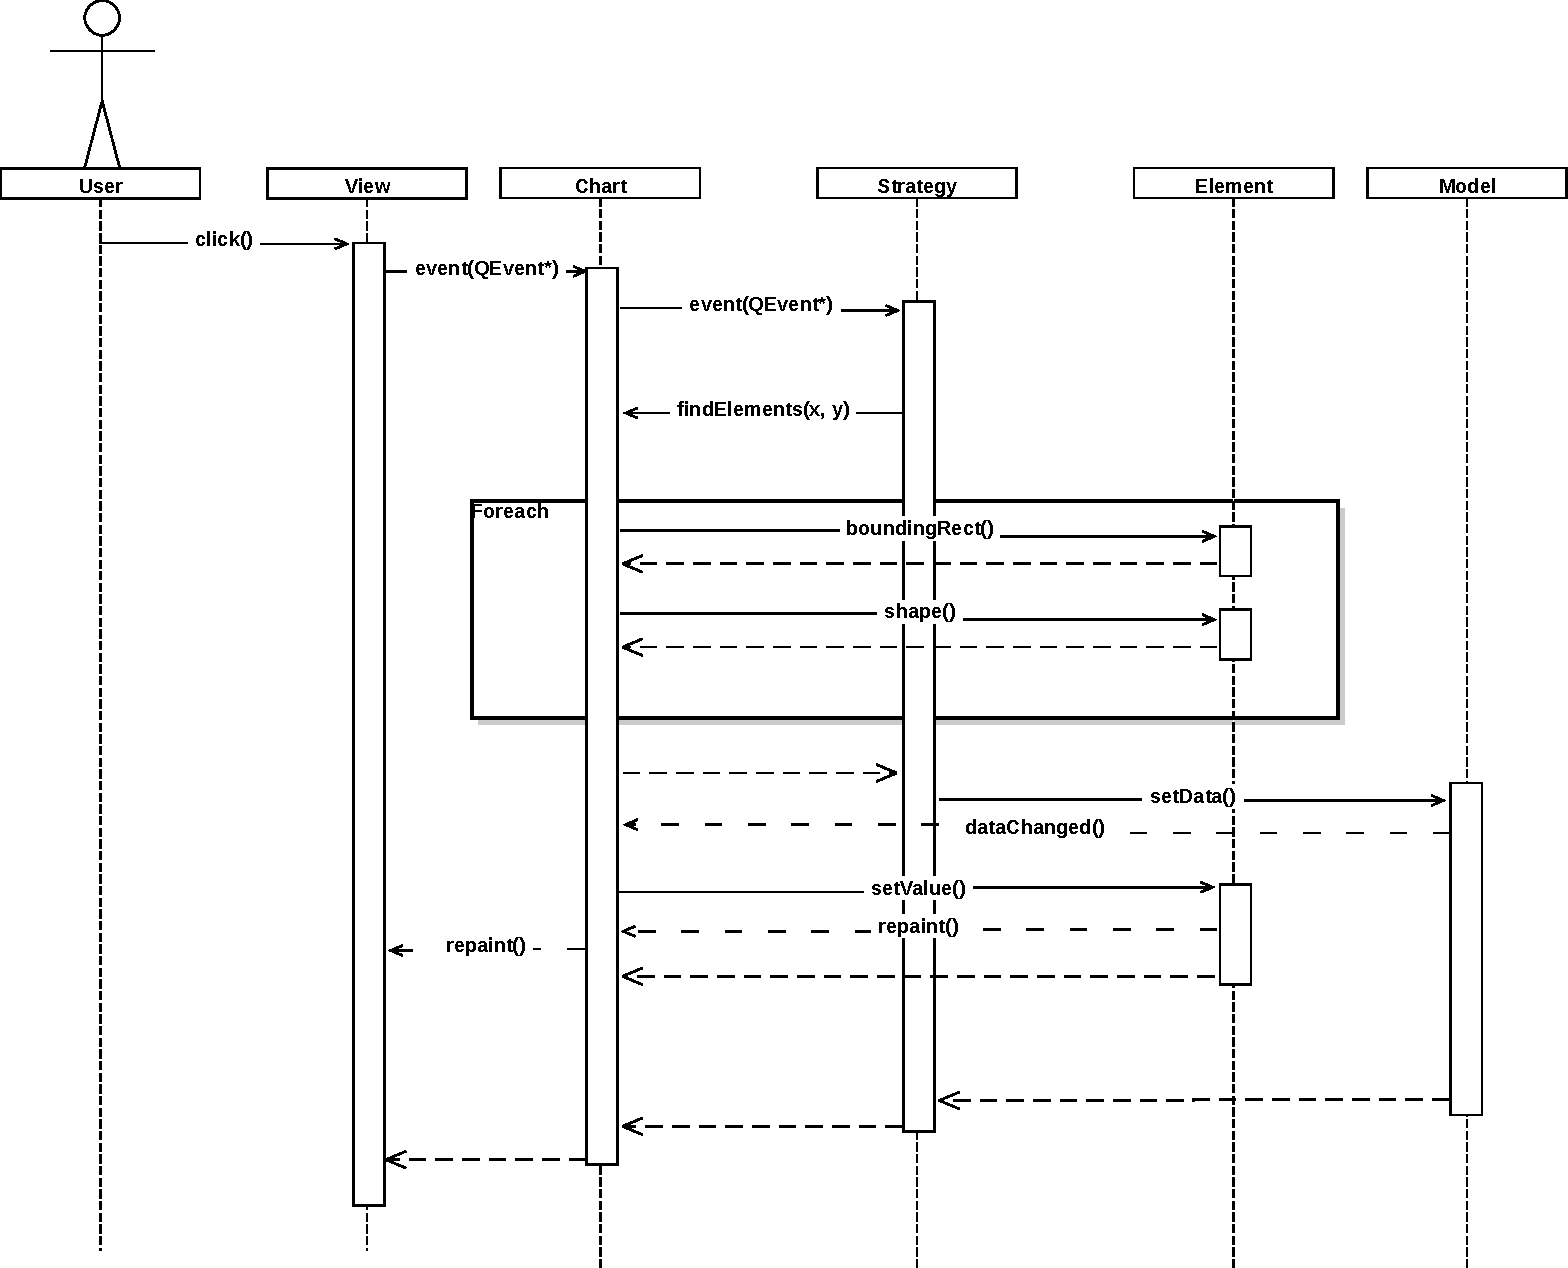
\includegraphics[scale=0.6]{img/seq_inter.pdf}
\caption{Interaktywna zmiana zawartości modelu}\label{rys:seq:inter}
\end{figure}

\section{Wykresy w układzie współrzędnych}
Większość wykresów jest osadzona w~pewnym układzie współrzędnych. Najpopularniejszym z~nich jest układ współrzędnych kartezjańskich~\ref{rys:uk:kart}, jednak jak wiadomo nie jest to jedyny układ współrzędnych. Moje rozwiązanie przewiduje możliwość tworzenia wykresów w~bardziej egzotycznych układach, np. wykres polarny w~układzie biegunowym~\ref{rys:uk:bieg}.

Mimo, iż najpopularniejszą skalą osi, stosowaną przy wykresach biurowych jest skala liniowa, moje rozwiązanie przewiduje możliwość wykorzystania innej skali, np. logarytmicznej, która jest dość często stosowana przy wykresach liniowych. 

\begin{figure}[H]
\centering
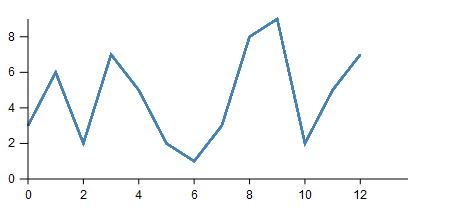
\includegraphics[scale=0.65]{img/kartezjanski.png}
\caption{Liniowy wykres w układzie kartezjańskim}\label{rys:uk:kart}
\end{figure}

\begin{figure}[H]
\centering
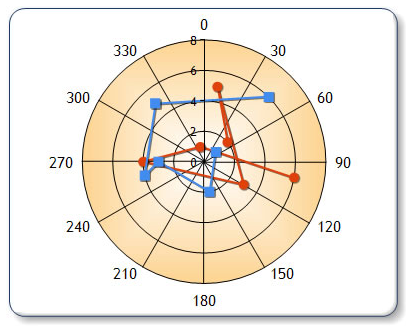
\includegraphics[scale=0.65]{img/biegunowy.png}
\caption{Wykres polarny}\label{rys:uk:bieg}
\end{figure}

Na diagramie~\ref{rys:os:skala} prezentuję hierarchię klas związanych z~układem współrzędnych. Jedyną klasą nie przewidzianą do dziedziczenia jest tu \textit{QocAxis}. Pozostałe elementy tej hierarchi powinny być dostosowywane do własnych potrzeb poprzez dziedziczenie.

\begin{figure}[H]
\centering
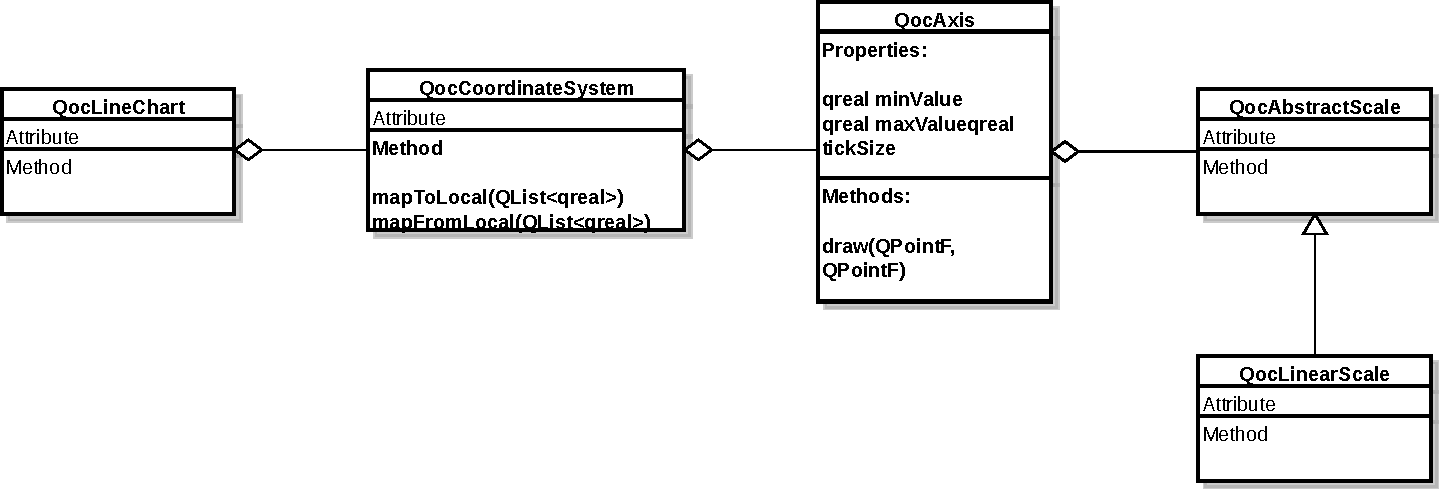
\includegraphics[scale=0.5]{img/os_skala.pdf}
\caption{Klasy związane z układem współrzędnych}\label{rys:os:skala}
\end{figure}

\subsection{Układ współrzędnych}
,,Układ współrzędnych -- funkcja przypisująca każdemu punktowi danej przestrzeni (w szczególności przestrzeni dwuwymiarowej -- płaszczyzny, powierzchni kuli itp.) skończony ciąg (krotkę) liczb rzeczywistych zwanych współrzędnymi punktu.''~\footnote{\url{http://pl.wikipedia.org/wiki/Układ\_współrzędnych}}

Głównym celem istnienia bytu o~nazwie \textit{QocAbstractCoordinateSystem} jest udostępnienie dwóch funkcji. Pierwsza z~nich przyjmuje wektor opisujący położenie punktu w~danej przestrzeni i~zwraca dwie współrzędne -- x~i~y tego punktu na płaszczyźnie wykresu. Druga funkcja działa dokładnie dokładnie odwrotnie. Takie podejście umożliwia dwukierunkowe mapowanie przestrzeni dwuwymiarowych, ale może być niewystarczające dla wykresów 3D. Poza opisaną funkcjonalnością, układ współrzędnych w~mojej bibliotece odpowiada również za zarządzanie osiami oraz odrysowywanie siatki.

\subsection{Osie i skale} 
Według mnie oś w układzie współrzędnych powinna być możliwie prostą i~niezmienną klasą, dlatego postanowiłem rozłączyć oś od jej skali -- jest to rozwiązanie podobne do zastosowanego w~Qwt~\footnote{Skala w Qwt \url{http://qwt.sourceforge.net/class\_qwt\_scale\_engine.html}}. Oś jest odpowiedzialna głównie za swoje odrysowywanie, pozostałe zadania związane z~wyliczaniem współrzędnych czy ticków oddelegowuje do swojej skali. Domyślną skalą jest skala liniowa, ale moje podejście umożliwia włączenie do biblioteki, np. skali logarytmicznej.

\section{Legenda}
Legenda jest elementem służącym do prezentacji dwóch właściwości: koloru oraz tytułu. W~zależności od typu wykresu są to właściwości pojedynczej próbki albo całej serii. 

Dodawanie legendy do wykresu odbywa się za pomocą metody \textit{QocAbstractChart::setLegend()}, która podłącza sygnały płynące ze źródła danych do obiektu klasy \textit{QocSignalMapper}. Zmapowane sygnały są podłączane do odpowiednich slotów legendy. Za pomocą specjalnego typu wyliczeniowego da się sparametryzować czy mapowanie ma zostać dokonane dla pojedynczych próbek czy dla całych serii. Cała koncepcja została zobrazowana na diagramie~\ref{rys:diag:legenda}.

\begin{figure}[H]
\centering
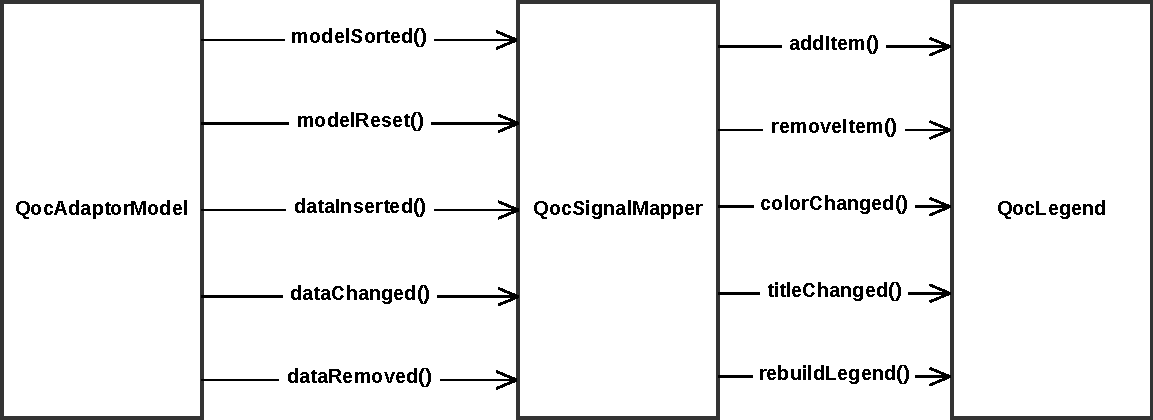
\includegraphics[scale=0.7]{img/legenda.pdf}
\caption{Komunikacja pomiędzy źródłem danych a legendą}\label{rys:diag:legenda}
\end{figure}

\subsection{Delegat}
Możliwość zmieny elementu prezentującego w~legendzie kolor rozwiązałem przez dodanie nowej właściwości legendy -- delegata. Musi to być obiekt klasy dziedziczącej po \textit{QObject}. Klasa ta musi posiadać metodę \textit{draw()}, jeśli korzysta z~\textit{QPainter}, albo \textit{updatePaintNode()} dla \textit{SceneGraph}. Podczas odrysowywania legendy wywoływana będzie jedna z~tych metod, korzystając z~systemu metadanych Qt -- \textit{QMetaObject::invokeMethod()}. Do tworzenia kolejnych instancji delegata wykorzystuję metodę \textit{QMetaObject::newInstance()}.  Dodatkowo delegat musi mieć właściwość ,,color''. Spełnienie tych kilku warunków sprawi, że programista będzie mógł wyświetlić w~legendzie kwadrat, trójkąt albo kwiatek. Domyślny delegat to element o~kształcie kwadratu.

\section{Współpraca wykresów z widokami }
Jak już zostało ustalone, celem tworzonej biblioteki jest stworzenie uniwersalnego silnika, umożliwiającego tworzenie wykresów gotowych do podpięcia do jednego z~kilku widoków. Na rysunku~\ref{rys:widok:wykres} przedstawiłem składniki protokołu komunikacji między widokiem a dowolnym wykresem z~mojej biblioteki.

Widok ma obowiązek przesyłać do wykresu wszelkie zdarzenia, które są dla niego przeznaczone oraz informować wykres o~zmianach swojej geometrii. Ponadto przy odrysowywaniu widok musi wywoływać metodę \textit{draw()} wykresu.

Wykres nie posiada informacji z~widokiem jakiej klasy współpracuje. Można to osiągnać za pomocą mechanizmu sygnałów i~slotów, który pozwala na luźne wiązanie elementów. Odpowiednie sygnały są emitowane przez wykres zawsze wtedy, gdy wymaga on ponownego odrysowania.
Sygnał \textit{repaint()} jest emitowany w~sytuacji, gdy ponowne odrysowanie musi nastąpić niemal natychmiast, natomiast sygnał \textit{update()} jest przeznaczony na sytuacje gdy zgłoszenia odrysowania mogą zostać skolejkowane, sklejone i~obsłużone jako jedno zgłoszenie w~najbliższej wolnej chwili.


\begin{figure}[H]
\centering
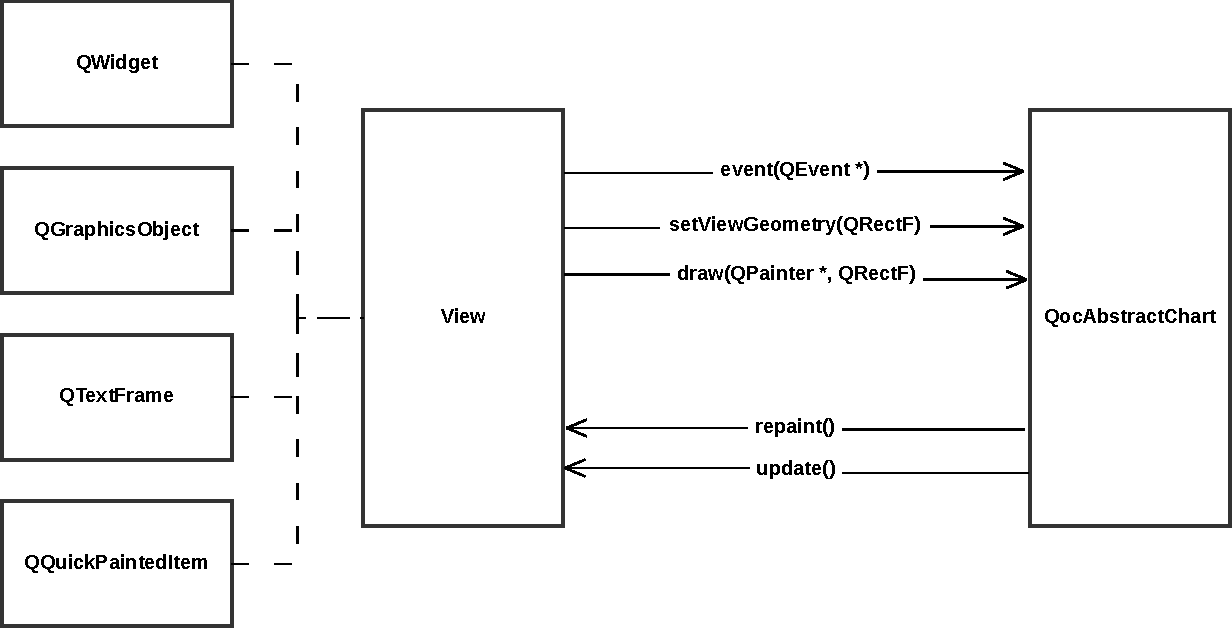
\includegraphics[scale=0.75]{img/widok-wykres.pdf}
\caption{Widok -- Wykres}\label{rys:widok:wykres}
\end{figure}

%\subsubsection{Wskazówki implementacyjne}
%Klasa bazowa wykresów powinna posiadać właściwość typu prostokąt, opisującą geometrię widoku podłączonego do danego wykresu. Zmiana tej właściwości powinna się odbywać poprzez odpowiedni slot, przyjmujący jako argument nowy prostokąt.

%W~zależności od klasy, z~której wywodzi się widok podłączony do wykresu, slot powiadamiający wykres o~zmianie geometrii widoku powinien być wywoływany następujących metodach widoku:
%\begin{itemize}
%\item{QWidget}
%	\begin{itemize}
%	\item{moveEvent()}
%	\item{resizeEvent()}
%	\end{itemize}
%\item{QGraphicsObject}
%	\begin{itemize}
%	\item{prepareGeometryChange()}
%	\end{itemize}
%\item{QTextFrame}

%\item{QQuickPaintedItem}
%	\begin{itemize}
%	\item{geometryChanged()}
%	\end{itemize}
%\end{itemize}

\section{Zależności między plikami}\label{sec:most}
Mogłoby się wydawać, że każde nowe wydanie Qt powinno wymagać ponownej kompilacji projektów zeń korzystających. Tak jednak nie jest. Twórcy Qt zadbali o~to, aby zawsze wtedy, kiedy to możliwe, zachowana była zgodność binarna. Oznacza to, że jeśli przy poprawkach do nowej wersji nie zostały zmienione nagłówki klas, a~jedynie ich implementacje, to przebudowanie całej aplikacji nie jest konieczne. Teoretycznie przejście z~Qt~w~wersji 4.8.3 na wersję 4.8.4 może odbyć się jedynie poprzez podmianę plików .dll. Temat zgodności binarnej oraz zależności czasu kompilacji między plikami został poruszony przez Scotta Meyersa~\cite{50Ways}.

\subsection{QObject}
Klasa QObject została zaprojektowana jako \textit{Most}~\cite{Patterns}.
%, zmodyfikowany o~posiadany przez ciało wskaźnik do uchwytu. 
Podział na uchwyt i~ciało zmniejsza zależności pomiędzy plikami bibliotek Qt i~znacząco skraca czas kompilacji po zmianach w~kodzie. Dodatkowo QObject posiada konstruktor przyjmujący jako argument wskaźnik do ciała, dzięki czemu można je zaalokować tylko raz, w~klasie najniższego poziomu hierarchii dziedziczenia, a~następnie przekazać jako argument konstruktora klasy bazowej. 
Koncepcję \textit{Mostu} zobrazowałem w~kontekście mojej biblioteki na rys.~\ref{rys:dpointer}.\newline

\begin{figure}[H]
\centering
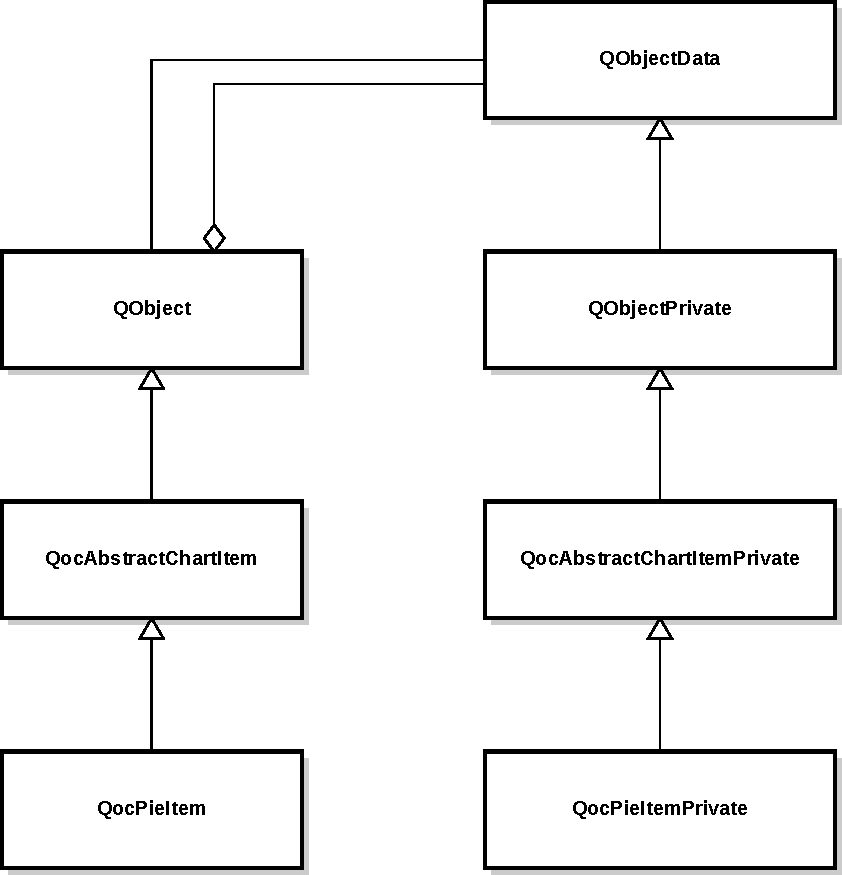
\includegraphics[scale=0.8]{img/dpointer.pdf}
\caption{Przykładowa hierarchia klas}\label{rys:dpointer}
\end{figure}

W~Qt przyjęto następującą koncepcję nazewniczą:
\begin{itemize}
\item{uchwyt ma standardową nazwę, zgodną ze swoim przeznaczeniem,}
\item{ciało ma nazwę składającą się z~nazwy odpowiadającego mu uchwytu oraz sufiksu ,,Private''.}
\end{itemize}


\subsection{Dostęp do uchwytów i ciał}

\begin{table}[h]\footnotesize
\centering
\caption{Makrodefinicje}
\label{tab:makra}
\begin{tabular}{|c|c|c|}
\hline
Miejsce & Uchwyt & Ciało\\
\hline
Nagłówek & Q\_DECLARE\_PRIVATE & Q\_DECLARE\_PUBLIC\\
\hline
Metoda & Q\_D & Q\_Q\\
\hline
\end{tabular}
\end{table}

Podejście opisane w~poprzednim punkcie skutkuje jednak powstaniem pewnego efektu ubocznego.
Wskaźniki do uchwytu i~ciała są typów klas znajdujących się na szczycie hierarchii dziedziczenia. Dostęp do metod klas pochodnych niewystępujących w~klasach bazowych wymaga rzutowania w~dół. 
Problem ten rozwiązano za pomocą czterech makrodefinicji przyjmujących jako argument nazwę klasy uchwytu. Dwie z~nich należy wywołać w~odpowiednich nagłówkach. Z~kolei pozostałe dwie należy wywoływać na początku każdej metody wymagającej odwołania do ciała lub uchwytu. Miejsce wykorzystania konkretnych makr podaję w~tablicy~\ref{tab:makra}. Technika ta została szczegółowo opisana w~artykule~\footnote{QObject -- Most \url{http://qt-project.org/wiki/Dpointer}}.


